Algoritmos como K-Means presentan dificultades para identificar clusters cuando las distancias entre elementos de un mismo conjunto es mayor que la de elementos de conjuntos distintos.
En estos casos, puesto que K-Means busca minimizar la distancia entre los elementos dentro de un mismo cluster, producirá clusters que difieran significativamente de los grupos <<correctos>>.
Podemos observar un ejemplo en el escenario de la figura~\ref{img:kmeans-dbscan}, donde se compara el resultado de K-Means con el del algoritmo que analizamos en esta sección, conocido como \textit{DBSCAN}.

\begin{figure}[!h]
    \centering
    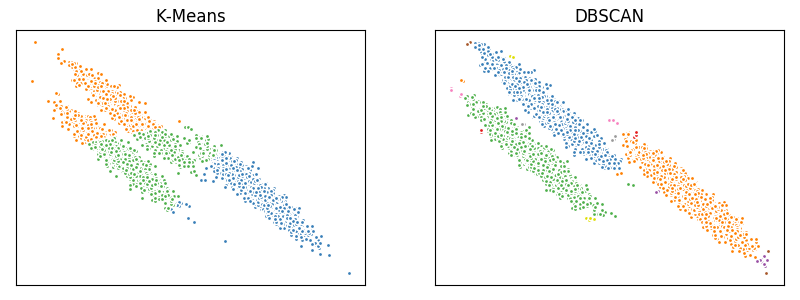
\includegraphics[width=\textwidth]{kmeans-dbscan.png}
    \caption{Resultados de los algoritmos K-Means y DBSCAN ejecutados sobre un conjunto de datos que sigue una distribución anisotrópica.}
    \label{img:kmeans-dbscan}
\end{figure}

En la imagen podemos observar asimismo el comportamiento de otro algoritmo sobre el mismo conjunto de datos.
En esta sección abordamos el algoritmo en cuestión, denominado \textit{DBSCAN}~\footnote{Siglas en inglés de \textit{Density-based spatial clustering of applications with noise}.}, que forma parte del conjunto de algoritmos de clustering basados en la densidad de los datos.

Un cluster basado en el criterio de densidad de los puntos consiste en un área densa de puntos conectados, separado de otros clusters por áreas de menor densidad.

\subsection{Densidad}\label{subsec:densidad}

El algoritmo DBSCAN define la densidad alrededor de un punto como la cantidad de puntos localizados alrededor de este en un radio, $Eps$, específico.
El propio punto es incluido en este conteo.
En la figura~\ref{img:dbscan} se puede observar gráficamente esta definición.
En este caso número de puntos alrededor de $A$ es 7.

El valor del radio es determinante en la densidad de un punto.
Si este valor es suficientemente grande, entonces todos los puntos tendrán una densidad de $n$, el número de puntos en el conjunto de datos.
En cambio, si el radio es demasiado pequeño, la densidad de todos los puntos será igual a 1.
Más adelante discutiremos algunas estrategias para la selección de valores apropiados para el radio. % TODO Check if accomplished

\begin{figure}[!h]
    \centering
    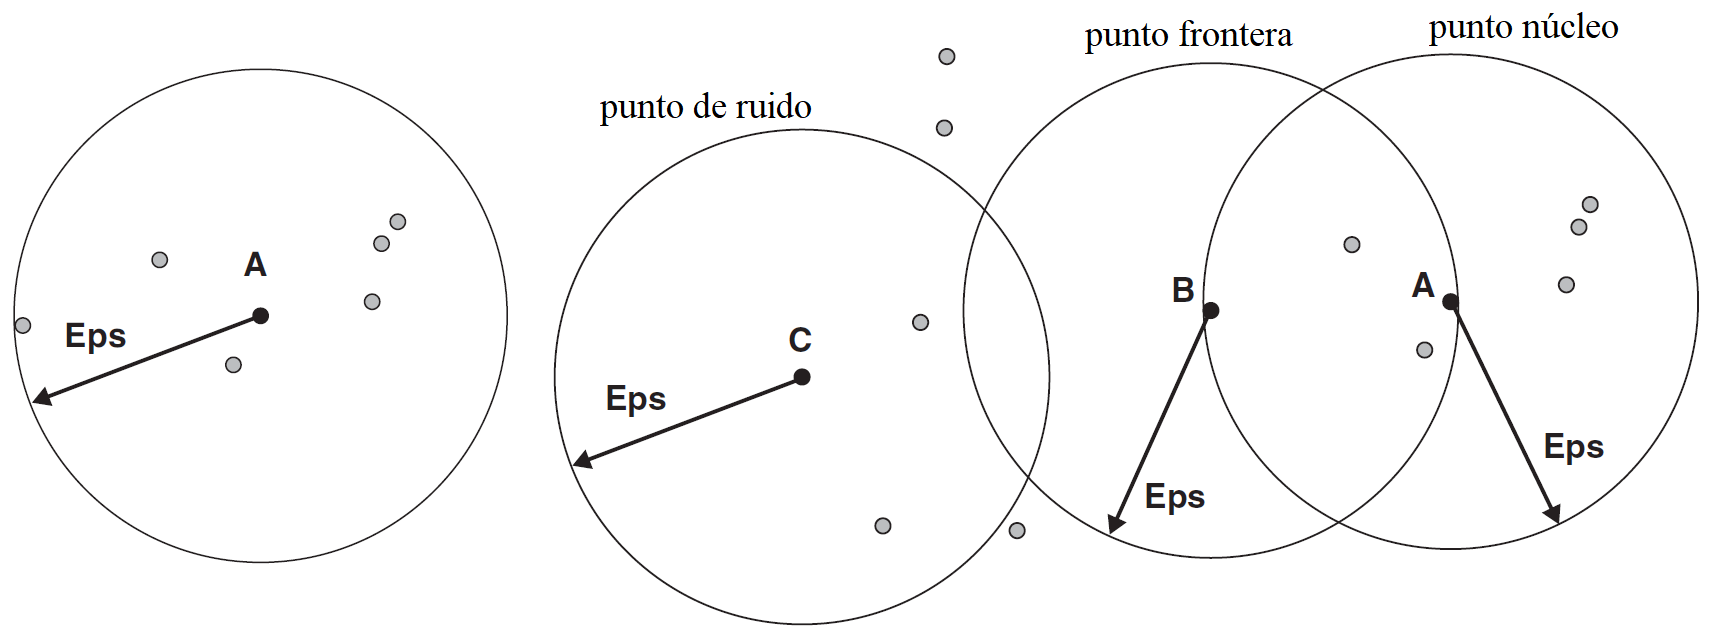
\includegraphics[width=\textwidth]{dbscan.png}
    \caption{Densidad en el entorno de un punto y clasificaciones de los puntos según su densidad.}
    \label{img:dbscan}
\end{figure}

De acuerdo con la densidad de un punto, estos pueden ser clasificados de la siguiente forma:

\begin{itemize}
    \item \textbf{Puntos núcleo}: Constituyen puntos de la región interna de un cluster basado en densidad. Un punto es núcleo si el número de puntos alrededor de este (incluyéndolo) supera o iguala un valor $MinPts$, especificado por el usuario. En la figura~\ref{img:dbscan} los puntos identificados con la letra $A$ son núcleos para el radio $Eps$ indicado si $MinPts\leq 7$.
    \item \textbf{Puntos frontera}: Un punto frontera es aquel que no cumple el criterio de núcleo, pero que forma parte de la vecindad de al menos uno de estos. En la figura~\ref{img:dbscan} $B$ es un punto frontera.
    \item \textbf{Puntos de ruido}: Un punto es de ruido si no es núcleo o frontera. En la figura~\ref{img:dbscan} $C$ es un punto de ruido.
\end{itemize}

\subsection{Algoritmo DBSCAN}

A partir de las definiciones dadas de puntos núcleos, fronteras y de ruido, podemos describir el algoritmo DBSCAN del siguiente modo: Todo par de puntos núcleos cuya distancia sea no mayor que $Eps$ son asignados al mismo cluster. De igual forma, los puntos fronteras son asignados al cluster de los puntos núcleos cuya distancia a estos sea menor o igual que $Eps$. (En caso de estar en la vecindad de núcleos pertenecientes a clusters diferentes, un criterio específico debe ser determinado al programar el algoritmo). Los puntos de ruido son descartados y no asignados a ningún cluster.